\documentclass[12pt]{article}
\usepackage{float}
\usepackage{times}
\usepackage{graphicx}
\usepackage{subfigure}
\usepackage{color}
\usepackage{url}
\usepackage{amsmath}
\usepackage{fixltx2e}
\usepackage{cleveref}
% ----------------------------------------------------------------------------
% Start the document
%
\begin{document}
  \begin{titlepage}
      \centering
      ~~~~~~~~~~~~~\\[-30mm]
      
\includegraphics[keepaspectratio=true, width=7cm]{bg_eng_1r.jpg} \\[10mm]

     {
     \large \bfseries Master Degree in Computer Science\\[3mm]
     Distributed Algorithms\\[3mm]
     AA 2015-2016
     }\\[10mm]

     % ------------------------------------------------------------------------
     % Set the title, author, and date
     %

     \vspace{0.5cm}
     {
     \Large \bfseries \textcolor{blue}{Community Detection using Giraph} \par
     }
     \vspace{0.5cm}
     {\large {Ardino Pierfrancesco, Natale Maria Pia, Tovo Alessia}}

     \vspace{0.3cm}

    % ------------------------------------------------------------------------
\begin{abstract}
    The content of this work is about the implementation of a Community Detection algorithm using a MapReduce framework.
    This report is created as course project of the Distributed Algorithms course held by prof. Alberto Montresor. A network is said to have \emph{community structure} if the nodes of the network can be grouped into sub-graphs such that these sub-graphs are densely connected internally. In the case of \emph{non-overlapping} communities, each node belongs to a single sub-graph or it is disconnected from the network if it does not belongs to none of them. \emph{Non-overlapping} communities have strong connections internally and weak connections with the other communities. There can be also \emph{overlapping} communities, here a node could belong to more than one community. It's straightforward to understand that \emph{overlapping} communities have stronger connections that the \emph{non-overlapping} ones.
Social networks are paradigmatic examples of graphs with communities. The word community itself refers to a social context. People naturally tend to form groups, within their work environment, family, friends.
    Detecting communities within a graph can be a difficult task. Decide whether a node has to belong to community instead of another one is not trivial. Also, typically the number of communities in a graph is unknown and so it can be difficult to understand if the found communities are correct or not. In this project we decided to implement the community detection algorithm developed in \cite{6517336}.
\end{abstract}

\end{titlepage}

\thispagestyle{empty}
\tableofcontents

\clearpage
\setcounter{page}{1}


    % ------------------------------------------------------------------------
    % This is where the body of the report begins; usually with an Introduction
    %
\section{Introduction}\label{Intro}
\subsection{Goals}
The aim of this work is to show a possible implementation of a community detection algorithm using a MapReduce framework. We made use of the Giraph framework in order to develop and test the proposed solution.
\subsection{Content}
The report is composed by many sections, firstly we will examine the algorithm described in \cite{6517336}; then we will describe our implementation of the algorithm and finally we will discuss the results of the algorithm in some graphs. In particular:
\begin{itemize}
    \item In the first chapter we will discuss the similarity metric used and the stages of the algorithm.
    \item In the second chapter we will firstly introduce Giraph and then discuss our implementation showing the messages exchanged by the nodes and the nodes structure.
    \item In the third chapter we will analyze the result obtained from the simulations and explain the different results obtained by varying the simulation parameters.
\end{itemize}

\section{Algorithm Overview}
The algorithm, which is called \emph{DEPOLD} (DElayed Processing of Large Degree Nodes),is composed of three Phases:
\begin{itemize}
    \item \emph{Preprocessing}
    \item \emph{Coreprocessing}
    \item \emph{Postprocessing}
\end{itemize}
        A new data structure called \emph{THALS} (Two-Hop Adjacency List with Similarity) is created specifically for the purpose of this MapReduce solution. This data structure is used as input and data format in parallel core-processing algorithms.
THALS is composed of the following fields:
\begin{itemize}
    \item Id of the vertex
    \item Adjacent list with similarity values which includes neighbor vertex Id and the corresponding similarity value between the vertex and his neighbor.
    \item Two-Hop adjacent list. The neighbors of a neighbor are stored using an hash table.
    \item label used to transmit information from Mapper to Reduced.
\end{itemize}
\subsection{Preprocessing}
In this phase the nodes with a degree larger than a specific threshold $\theta$ are found. This is done because nodes with a large degree can cause a bottleneck during the phase of \emph{Coreprocessing} and can confuse the structure of a community. These nodes are disabled and re-enabled in the Postprocessing phase.
\subsection{Coreprocessing}
In this phase the similarity value between the linked vertices is iteratively computed. The link will be removed if the similarity value is less than a specific threshold $\gamma$. When the change of the topology is less than a threshold $\varphi$ the algorithm has converged.\\
The similarity between two nodes is computed as following:

\begin{equation}
    S(v\textsubscript{i},v\textsubscript{j}) =
  \begin{cases}
      \frac{1 + C(v\textsubscript{i},v\textsubscript{j}) + \eta(v\textsubscript{i},v\textsubscript{j}) } {F(v\textsubscript{i},v\textsubscript{j}) }       & \quad \text{if } \left|E(v\textsubscript{i},v\textsubscript{j}) \right| = 1\\
              0  & \quad \text{ otherwise}\\
                \end{cases}
    \label{eq:1}
\end{equation}
where $C(v\textsubscript{i},v\textsubscript{j})$ is the number of common neighbors between $v\textsubscript{i}$ and $v\textsubscript{j}$, $\eta(v\textsubscript{i},v\textsubscript{j})$ is the number of the edges between the common neighbors of  $v\textsubscript{i}$ and $v\textsubscript{j}$ and $F(v\textsubscript{i},v\textsubscript{j})$ is the sum of the degree of
$v\textsubscript{i}$ and $v\textsubscript{j}$.
\subsection{Postprocessing}
In this phase the communities division are found by discovering the \emph{Weakly Connected Components}. Then the high-degree nodes are merged in a community by computing the degree the filtered node contributes to that community and the average contributed degree of the detected community members. It can be that the filtered nodes can belong to more than one communities, in this case the algorithm stores each community to which the node belongs. Finally an hash map containing the Id of the node and the Id of the community to which it belongs is written to the HDFS.
\section{Implementation}
\subsection{Giraph}
\texttt{Giraph} is a synchronous iterative graph processing framework, originated as the open-source counterpart to \texttt{Pregel} and built on top of \texttt{Apache Hadoop}.
The input to a Giraph computation is a graph composed of vertices and directed edges. Computation proceeds as a sequence of iterations, called \emph{supersteps}. Initially, every vertex is \emph{active}. In each superstep each active vertex invokes the \emph{Compute method} provided by the user. The method implements the graph algorithm that will be executed on the input graph.
The Compute method dose the following operations:
\begin{itemize}
    \item receives messages sent to the vertex in the previous superstep
    \item computes using the received messages and the vertex value which may result in a modification to the vertex itself
    \item may send messages to other vertices.
\end{itemize}
    The Compute does not have knowledge of the values of the other vertices. It can retrieve information of the other vertices through Inter-vertex communication by exchanging messages.
    The computation halts after the vertices have voted to halt and there are no messages in flight.
\subsection{Structure of the code}
The classes developed for this project are the following:
\subsubsection{Node}
    This class stores information about a node in the Two-Hop adjacent list and in the Similarity map.
    The class is composed of two fields:
    \begin{itemize}
            \item \emph{Long} ID
            \item \emph{Boolean} active
    \end{itemize}
    The ID field contains the Id of a node while the active field, which is initialized to \emph{true}, contains the status of a node.
\subsubsection{Node\_Degree}
This class stores information about the degree of a node.
The class is composed of two fields:
\begin{itemize}
    \item \emph{Long} ID
    \item \emph{Long} Degree
\end{itemize}
    The ID field contains the Id of a node while the Degree field, contains the degree of a node.
    In the case of filtered nodes, the ID field is used to store one of the community of the node.
\subsubsection{THALS}
This class implements the THALS data structure with some changes.
The class is composed of the following fields:
\begin{itemize}
    \item \emph{Map$<$Node,Node$>$} two\_hop
    \item \emph{Boolean} active
    \item \emph{Long} group\_id
    \item \emph{ArrayList$<$Node\_Degree$>$} community\_members
    \item \emph{Map$<$Node, DoubleWritable$>$} similarity\_map
    \item \emph{ArrayList$<$Node\_Degree$>$} community\_filtered\_node
\end{itemize}
    The \emph{two\_hop} field contains the two-hop adjacent list of a node, the \emph{active} field contains the status of a node, the \emph{group\_id} field contains the community Id of a node, the \emph{community\_members} field contains the list of nodes which belong to the same community of the node, the \emph{similarity\_map} field is a map containing as key the neighbor of a node and as value the similarity value between the two nodes, the \emph{field community\_filtered\_node} contains the list of communities to which a filtered node belongs.
    The two\_hop, group\_id, community\_members, similarity\_map fields are used only by the non filtered nodes.
    We decided to use an ArrayList to store the communities of a filtered node because it can be possible that the node belongs to more than one community.
\subsubsection{DepoldInputFormat}
This class is used to load the raw data and initialize the vertices and create the edges.
Here we specify the type of the Id of the Vertex, \emph{LongWritable} in our case, the type of the data of the Vertex, \emph{THALS} in our case and the type of the data of the Edge, \emph{FloatWritable} in our case.
\subsubsection{DepoldOutputFormat}
This class is used to write the result of the algorithm to the HDFS, in the case of non filtered nodes it prints the \emph{Id} of the nodes and the \emph{group\_id}, while in the case of filtered nodes it prints the \emph{Id} of the nodes and the list of their communities.
\subsubsection{DepoldMaster}
The \emph{Compute method} of this class is the first thing that gets executed in a superstep, so it useful in combination of \emph{Aggregators} to manage the steps of the algorithm. An \emph{Aggregator} is used to check whether a global condition is satisfied or to keep some statistics. During a superstep, vertices provide values to aggregators. These values get aggregated by the system and the results become available to all vertices in the following superstep. We use five Aggregators to manage the phases of the algorithm, keeping track of how many nodes were filtered, keeping track of how many edges are deleted in the \emph{Coreprocessing} in order to check if the algorithm has converged, check if the \emph{WeaklyConnectedComponents} has converged and check if each node knows each node belonging to its community.
\subsubsection{MessageWritable}
This class is used to store the information exchanged between vertices. This class contains every kind of message that can be exchanged.
It is composed of the following fields:
\begin{itemize}
    \item \emph{Long} ID
    \item \emph{LongArrayList} neighbors
    \item \emph{Boolean} active
    \item \emph{LongArrayList} deleted\_nodes
    \item \emph{Long} group\_id
    \item \emph{ArrayList$<$Node\_Degree$>$} community\_members
\end{itemize}
    The \emph{ID} field contains the sender of the message, the \emph{neighbors} field contains the neighbors of the sender, the \emph{active} fields contains the status of the sender, the \emph{deleted\_nodes} field contains the node deleted by the sender in the \emph{Coreprocessing},
    the \emph{group\_id} field contains the community of the sender, the \emph{community\_members} field contains the list of nodes belonging to the community of the sender.
\subsubsection{Depold}
This is the most important class and the core of the system. The algorithm has 3 Stage divided into 14 phases. In the following section we will deeply describe each phase of the algorithm.
\subsection{Preprocessing}
\subsubsection{Preprocessing\_Two\_Hop\_First\_Phase}
In this phase we compute the adjacency list of the node and send it to its neighbors.
\subsubsection{Preprocessing\_Two\_Hop\_Second\_Phase}
Since we expect that the input is an undirected graphs, in this phase we first check if the \emph{Id} of the senders of the messages are already in the neighbors list of the nodes, if they are not present we add them to the list in order to complete the undirected graph.
Then we forward the adjacency list received from its neighbors to all its neighbors so each node will know the neighbors of his neighbors.
\subsubsection{Preprocessing\_Two\_Hop\_Third\_Phase}
In this phase we firstly compute the \emph{Two\_hop\_map} of the node, then we filter the nodes with a degree larger than the threshold $\theta$ setting the \emph{active} field to \emph{false} and finally send the status of the node to its neighbors.
\subsubsection{Preprocessing\_Second\_Phase}
In this phase we simply deactivate the edges that connect an unfiltered node to a filtered node by setting the \emph{active} field of the key or of the value of the \emph{Two\_hop\_map} to \emph{false}.
\subsection{Coreprocessing}
\subsubsection{Coreprocessing\_Similarity\_Phase}
In this phase we compute the similarity between a node and its active neighbors and put the values in the \emph{Similarity\_map}. We have noticed that the result of \Cref{eq:1} differs from the result of the algorithm used in the \emph{Coreprocessing} of \cite{6517336} in particular the \emph{CMPI S\_Calculator} which is showed below:
     \begin{figure}[H]
       \centering
         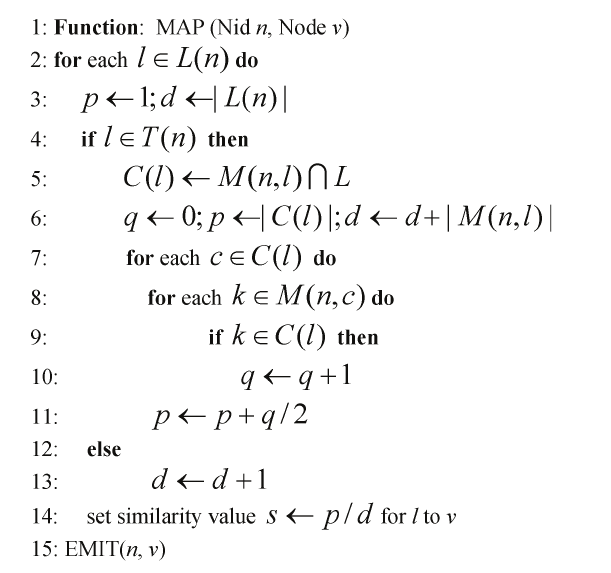
\includegraphics[width=0.7\textwidth]{similarity-code.png}
       \caption{CMPI S\_Calculator algorithm}
       \label{fig:depold}
     \end{figure}
We decided to use this algorithm to compute the similarity with another change. In fact, we have noticed that
if $v\textsubscript{i}$ and $v\textsubscript{j}$ do not have common neighbors $S(v\textsubscript{i},v\textsubscript{j})$ can differ from  $S(v\textsubscript{j},v\textsubscript{i})$. I.e. if $v\textsubscript{i}$ has 3 neighbors and $v\textsubscript{j}$ has 2 neighbors but they do not have common neighbors the result using the algorithm would be:
\begin{equation}
  S(v\textsubscript{i},v\textsubscript{j}) = \frac{1}{1 + d} = \frac{1}{4} = 0.25
\end{equation}
\begin{equation}
  S(v\textsubscript{j},v\textsubscript{i}) = \frac{1}{1 + d} = \frac{1}{3} = 0.33
\end{equation}
while they should be equal.This can potentially change the graph in an undirected one if   $S(v\textsubscript{i},v\textsubscript{j})$ is under the $\alpha$ threshold and $S(v\textsubscript{j},v\textsubscript{i})$ is over.
We decided to use the minimum between the number of neighbors of the two nodes plus 1. So line 13 of the algorithm becomes
\begin{equation}
    d = 1 + min(\pi(i), \pi(j))
\end{equation}
where $\pi(i)$ is the number of neighbors of $v\textsubscript{i}$ and $\pi(j)$ is the number of neighbors of $v\textsubscript{j}$
\subsubsection{Coreprocessing\_Topology\_First\_Phase}
In the phase we check if the similarity values in the \emph{Similarity\_Map} are under the $\alpha$ threshold. If so we delete the edges connecting the nodes, delete the entries in both \emph{Two\_Hop\_map} and \emph{Similarity\_map}, updates the Aggregator that takes track of the deleted nodes and finally send the \emph{Deleted\_nodes} list to the neighbors of the nodes.
\subsubsection{Coreprocessing\_Topology\_Second\_Phase}
In this phase we check if there are nodes in the \emph{Deleted\_nodes} list sent by the neighbors of the nodes that have to be deleted in the \emph{Two\_Hop\_map}. In fact, it can be that some edges representing an entry in the \emph{Two\_Hop\_map} no longer exists and so we have to delete that entry. If at the end of this phase the number of deleted nodes is over the $\varphi$ threshold, we return to the beginning of the \emph{Coreprocessing} stage.
\subsection{Postprocessing}
\subsubsection{Postprocessing\_WCC\_First}
In this phase we initialize the algorithm to compute the \emph{Weakly Connected Components}. This algorithm is used to find the communities of the unfiltered nodes.
\subsubsection{Postprocessing\_WCC\_Ssecond}
In this phase we compute the WCC and we assign a \emph{group\_id} to each unfiltered node. The \emph{Postprocessing\_WCC} phase converges if no vertices change community.
\subsubsection{Postprocessing\_Degree\_Calculator\_First}
In this phase we add to the \emph{Community\_members} list all the active neighbors of a node and then we send this list to neighbors of the nodes.
\subsubsection{Postprocessing\_Degree\_Calculator\_Second}
In this phase we add to the \emph{Community\_members} list all nodes received from the neighbors of a node which are not already in the list. Once we add the nodes to the list we send again the list to the neighbors of the nodes. The \emph{Postprocessing\_Degree\_Calculator} phase converges if no more nodes are added to the \emph{Community\_members} list.
\subsubsection{Postprocessing\_Degree\_Calculator\_Third}
In this phase we send the \emph{Community\_members} list to the neighbors which have been filtered in the \emph{Preprocessing} stage.
\subsubsection{Postprocessing\_Group\_Detector}
In this final phase the filtered nodes are merged into the existing communities. As said before, a filtered node can belong to more than one community. A filtered node belongs to a community if the number of its neighbors which belong to the community is larger than the average degree of that community. At the end of this stage, each unfiltered node has the \emph{group\_id} of the community to which it belongs, while each filtered node has the \emph{community\_filtered\_node} list of the communities to which it belongs.
\section{Simulations and Results}
\subsection{Assumption}
The assumption made for the project are the following:
\begin{itemize}
    \item the \emph{Id} of a node is an Integer value
    \item the \emph{group\_id} of a node is the smallest \emph{Id} of a \textbf{unfiltered }node in that community
    \item if all node are filtered than all node belong to the same community
\end{itemize}


\section{Results}\label{results}
\section{conclusions}
\label{conclu}

\bibliographystyle{ieeetr}
\bibliography{biblio}
    %
%    \appendix
%    \chapter{}

    % \printindex

\end{document}
